\section{Application}
\label{Application}
	\subsection{Information Procurement}
	The main theme of the collected data would concentrate around the topic of Internet Sales Platforms also known as E-Commerce. Several aspects make the topic beneficial for this research. Firstly,  such companies are almost exclusively web-based. It is therefore probable that most of the company's marketing efforts as well as overall news relating to such a firm, would circulate first and foremost in the Internet. Secondly, all company-relevant news are attainable from the web before all other resources. Hence, such news will in all likelihood seep to social media faster than announcements and other stories, which are predominantly covered by traditional media such as television and Newspapers. Therefore, the E-Commerce theme is likely to be widely and swiftly covered on social media, which is beneficial for the purposes of this study, since social media is used as the source of all data.
	
		\subsubsection*{Search Terms}
			The data was collected in the form of relevant Tweets from the Twitter Stream API. A Tweet would be considered relevant if it contained a search parameter related contextually to E-Commerce. The initial efforts were concentrated around the web-store Amazon. \textbf{Amazon} appears to the most fruitful search parameter, in terms of the quantity of Tweets relating to it. Additional search words that were tested were {\bfseries Alibaba, Zalando} and {\bfseries Groupon}, but proved to be impractical due to less data. 
			
			\par
			
			The widespread mention of Amazon in Tweets is somewhat over-inflated due to the extensive use of Amazon gift cards. Amazon gift-cards have become preponderate owing to their variety of uses. A few examples of common practices involving Amazon gift cards are rewarding users for services, such as polls and questionnaires, enticing people to take part in events or groups, and being offered as general rewards in competitions and games. The plethora of uses, facilitates Amazon gift cards to be viewed as a sort of pseudo-currency in the Internet. In turn this means, that Amazon could be mentioned in a Tweet, despite the context only indicating the Gift-card and being completely unassociated to the E-Commerce platform directly. Such Tweets are generally less valuable for the purpose of gaining knowledge about Amazon itself.
		
		\subsubsection*{Collecting the Data}
		\label{sec:collect_data}
			The gathering of Tweets was executed using a program written in the Python programming language for the purpose of this research. All software created for this project is available on \href{https://github.com/burningskies42/Twitter_Analytics}{\textit{GitHub}} \footnote{\url{https://github.com/burningskies42/Twitter_Analytics}}. A wrapper module called \textit{Tweepy}\footnote{\url{http://tweepy.readthedocs.io/en/v3.5.0/}} was implemented for interacting with the Twitter Streaming API. Tweepy is an open source interface, which allows communicating with the Twitters servers and sending queries requesting specific information from Twitter's databases. The interface allows for two main type of queries, \textit{Rest} and \textit{Streaming}. The former scans the servers for information posted on Twitter in the past whereas the latter, as the name implies, connects to an active data stream containing a narrowed down flow of Tweets being actively published by Twitter users. Both types of API's are being offered for free to a certain extent, whereas almost unrestricted versions of the same API are offered as a proprietary fee-based product of Twitter. The free version of the REST API is restricted to looking up Tweets posted in the last two to three weeks. Similarly, the gratis version of the Streaming API is restricted to a fire-hose narrowed down to about 15\% of the total Bandwidth of all current Tweets.
			
			\par
			
			The data units incoming from the Twitter servers are sent as JavaScript Object Notation (JSON) strings. JSONs are structured hierarchically, which allows for embedding other JSON objects in them recursively. This makes JSON beneficial for Tweets, since it allows multi-level storage of Tweet propertries and objects. For example, one of the JSON objects integrated in each Tweet JSON is the USER object for the Tweet-poster. A USER object, a JSON by itself, contains all relevant data for a Tweeter account. The USER object in turn contains all data publicly available in Twitter about a Twitter account such as, location, date of registration, homepage etc. An additional object of interest is the ENTITIES JSON object, which contains all outside references from the Tweet's text such as, URLs, Multimedia, References to other Tweets or other users. 
			This structure greatly eases the analysis of a Tweet and its features, since most of the necessary data is available from the Tweet itself and no further queries about the Tweets and its posting-user are necessary.
			\par
		
		\subsubsection*{Data cleansing}
			It was observed that numerous Tweets were being posted more than once and in several occurrences even hundreds of times. These duplicates were being primarily posted by bots, as was evident from a short observation of user profiles belonging the Tweets original posters. Evidently, additional effort was being made by the programmers of the bots to try and mask them by slightly altering the content of the Tweets, or the user account. This was usually done by changing or adding characters to the text, which carry no lingual significance in themselves. Moreover, in furtherance of increasing the bots' credibility as an actual people, often times entire nets of such bot could be observed, wherein the bots would maintain friendship and following connections among themselves. An example is shown in figure \ref{fig:twitterbot}. This in turn, increases the amount of \textit{friends} and \textit{followers}, further contributing to their guise of real human users of Tweeter. Upon closer observation, such accounts reveal their true essence, since most of the content propagated by them is commercial in nature and is repeated verbatim time and again across many of the related accounts \textit{followers} and \textit{friends}. For this reason, it is safe to assume that no actual people are behind these accounts. 
		\par
		
		\begin{figure}[h]
			\centering
			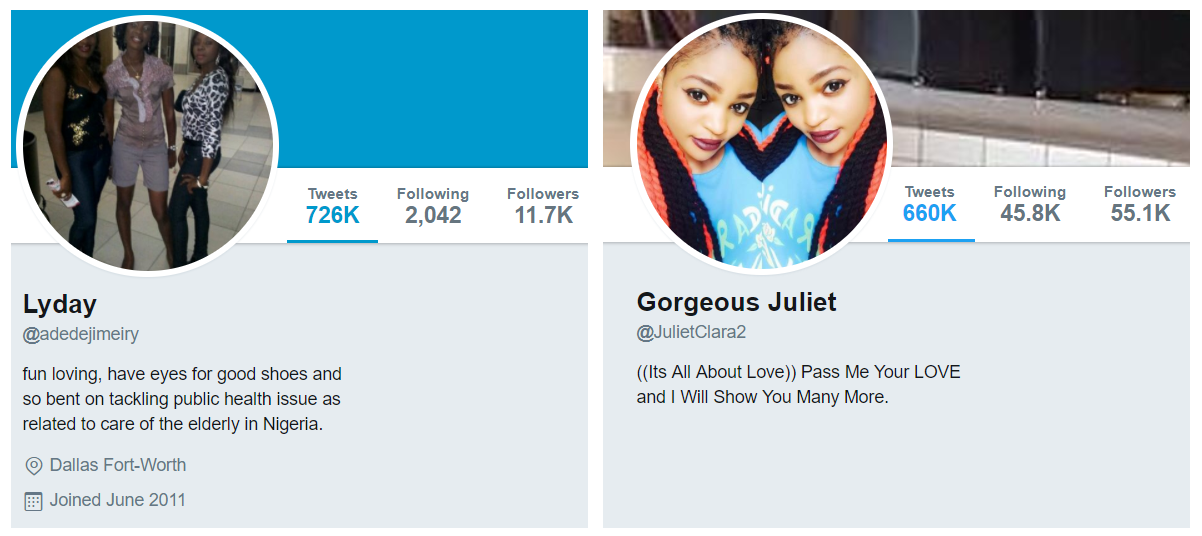
\includegraphics[width=0.8\textwidth]{twitterbot.PNG}
			\captionsetup{width=0.8\textwidth}
			\caption[Fake Twitter Accounts]{Twitter accounts, which present themselves as actual people}
			\label{fig:twitterbot}	
		\end{figure}
		
		\noindent
		Several precautions were undertaken to try and filter out such bots. A passive precaution which was implemented, was blacklisting users, which had priorly been observed posting Tweets, which were verbatim copies of other Tweets within the same query. The suspected users were added to a suspect database and content originating from them was ignored in future queries. Another action undertaken with the same purpose in mind was a retrospective cleanup of the collected Tweets, based on their content similarity. After closing a collection query, a maximum similarity measure for each Tweet in relation to all other recorded Tweets was calculated using a simple rule. Following, Tweets which were found to have a maximal similarity score to other previously captured Tweets  higher than a predetermined threshold were classified as non-unique copies and were disregarded. As a measure of similarity, the S\o rensen-Dice coefficient \cite{sorensen1948method} was implemented  using the \textit{SequenceMatcher.ratio()} function from the difflib Python module. The coefficient is demonstrated in figure \ref{fig:sorenson_dice} where $|X|$ and $|Y|$ are the numbers of elements in given Tweets X and Y accordingly. A higher $ QS_{XY} $ value indicates larger conformity between the $ X $ and $ Y $ groups, and ranges from 0 (completely different) to 1 (identical). A round of cleanup using this procedure would usually reduce a data set by from one quarter and up to one half of its original size.
		
		\begin{figure}[h]
			\begin{center}
				$QS_{XY} = \dfrac{2|X\cap Y|}{|X|+|Y|},$ \hspace{10pt}  $QS_{XY} \in [0:1]$
			\end{center}
			\caption{S\o rensen-Dice coefficient}
			\label{fig:sorenson_dice}
		\end{figure}
		
	\subsection{Building Feature-Sets}
	\label{build_features}
	Once a list of labeled Tweets is obtained, the next stage is constructing a feature-set to be later passed on as input for training an ML Classifier. The features contained if the feature sets describe certain aspects and characteristics of a Tweet and its owner. Two main approaches to feature sets are \textit{Word-Based} also often called \textit{Bag-of-Words} and \textit{Descriptive}. A further modification on \textit{Bag-of-Words} is \textit{N-Grams}. The different approaches to feature extraction are discussed in detail in section \ref{section:feature_types}.
	
			
	\subsection{Training Classifiers}
		Several configuration are to be applied when training the different classifiers, in the interest of quantifying and measuring the quality of classification. Hence, the size of the datasets used for training will vary, to observe the relation between set size and classifier accuracy. Additionally, different amounts of features should be tested, to determine whether accuracy grows linearly as the number of features increase or rather converges after some threshold. Furthermore, the training duration is to be measured to determine effectiveness of training as a time function.
		
		\par
		
		The different classifiers are grouped according to their designation and type as discussed in \hyperref[classifer_types]{section 3.2}. Additionally, another classifier type is one, which incorporates all previous classifiers and classifies with a majority vote. This classifier will be referred to as Vote Classifier. An apparent drawback of the Vote Classifier, is the classification duration which will be as long as the sum of classification durations of all its components.
		
		